\documentclass[12pt,a4paper]{article}

\usepackage{graphicx}  % permite adicionar figuras
\usepackage[utf8]{inputenc}  % permite acentuacao
\usepackage[portuguese]{babel}  % traduz palavras da formatacao

\begin{document}
\section{Ambiente matem\'atico}
Teorema de Pit\'agoras: $a^2=b^2+c^2$.
Teorema de Pit\'agoras: \[a^2=b^2+c^2.\]
Teorema de Pit\'agoras:
\begin{equation}
    a^2=b^2+c^2.
\end{equation}

\section{Figuras}
\begin{figure}[h]
    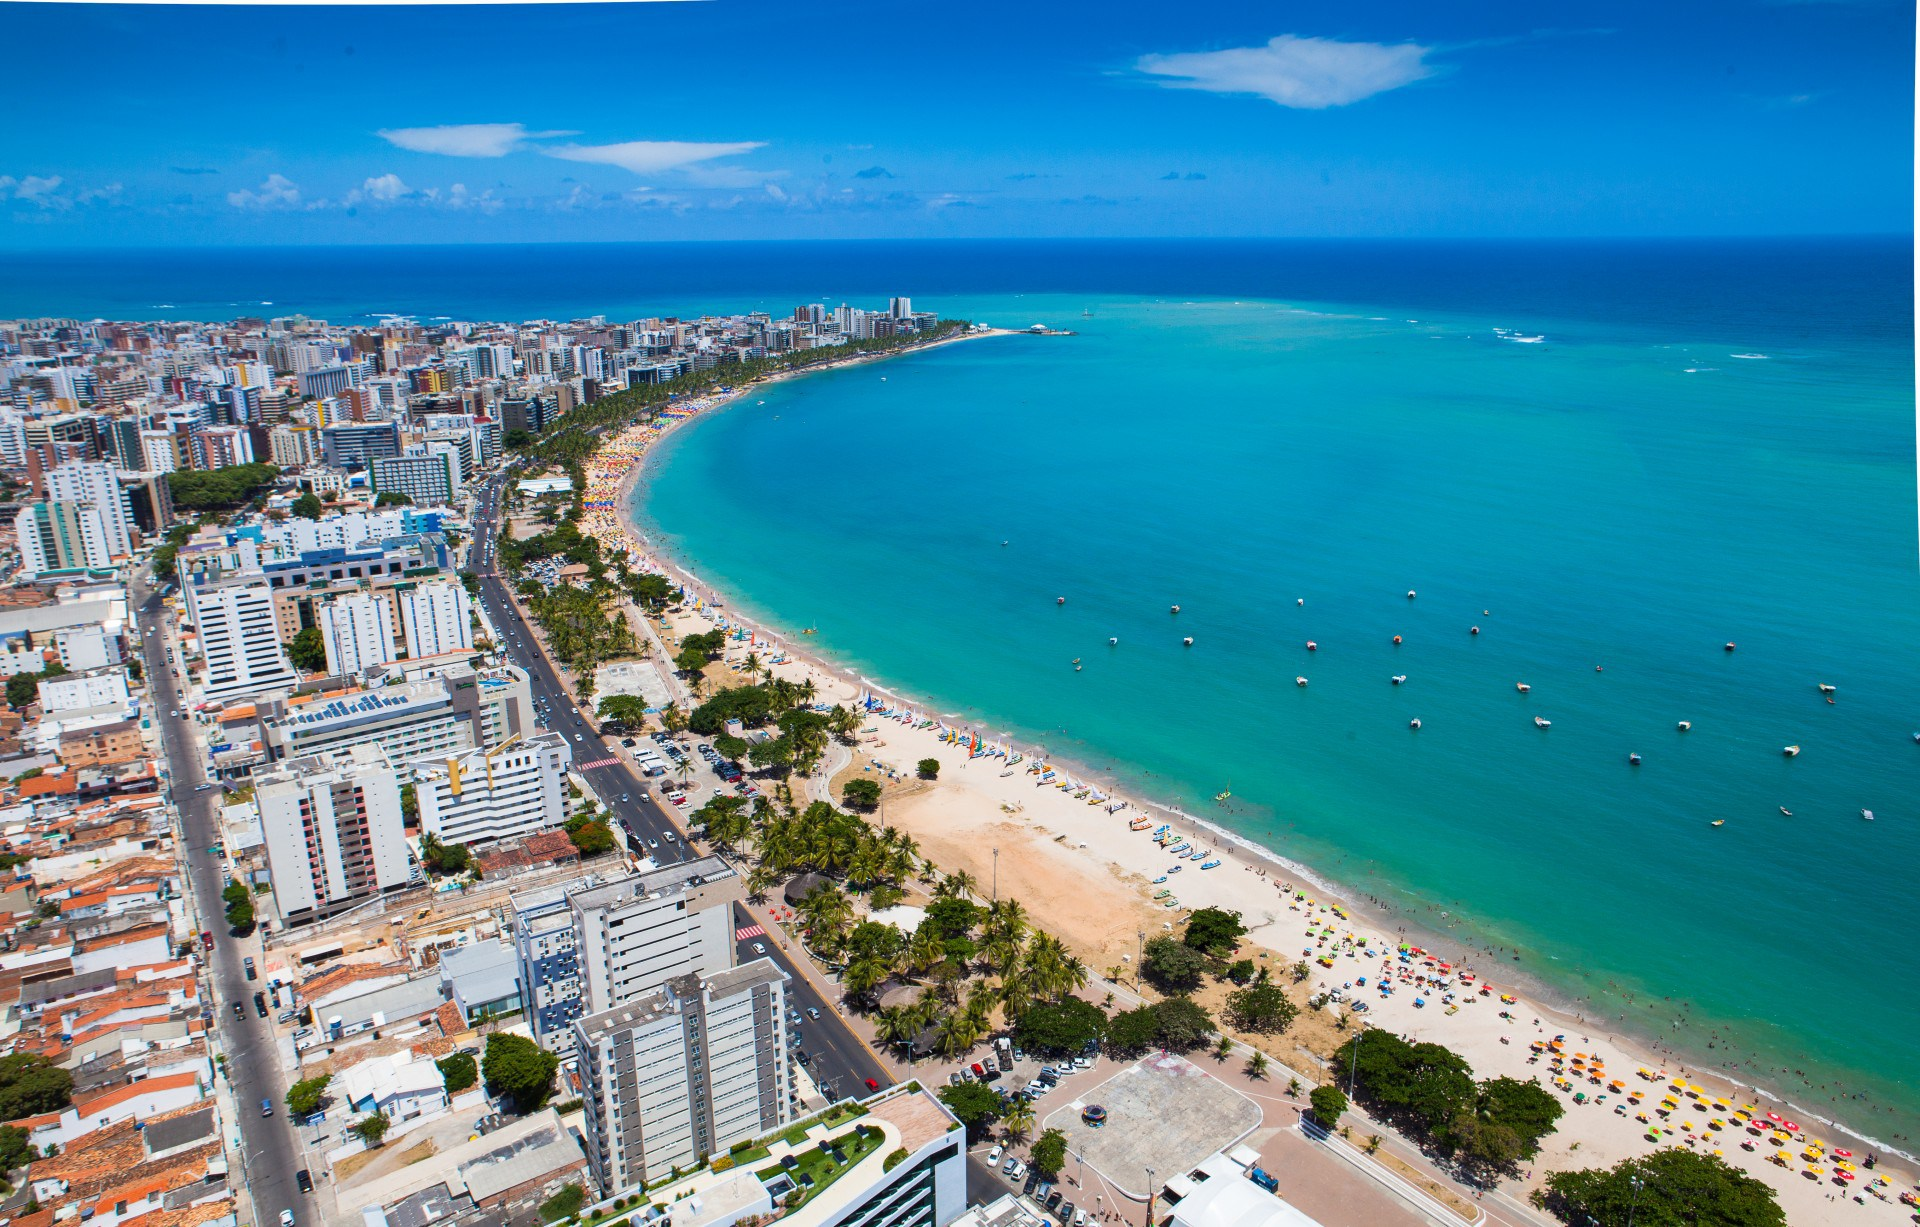
\includegraphics[scale=0.1]{maceio.jpg}
    \caption{Para\'{\i}so das \'aguas.}
\end{figure}
\begin{figure}[h]
    \centering
    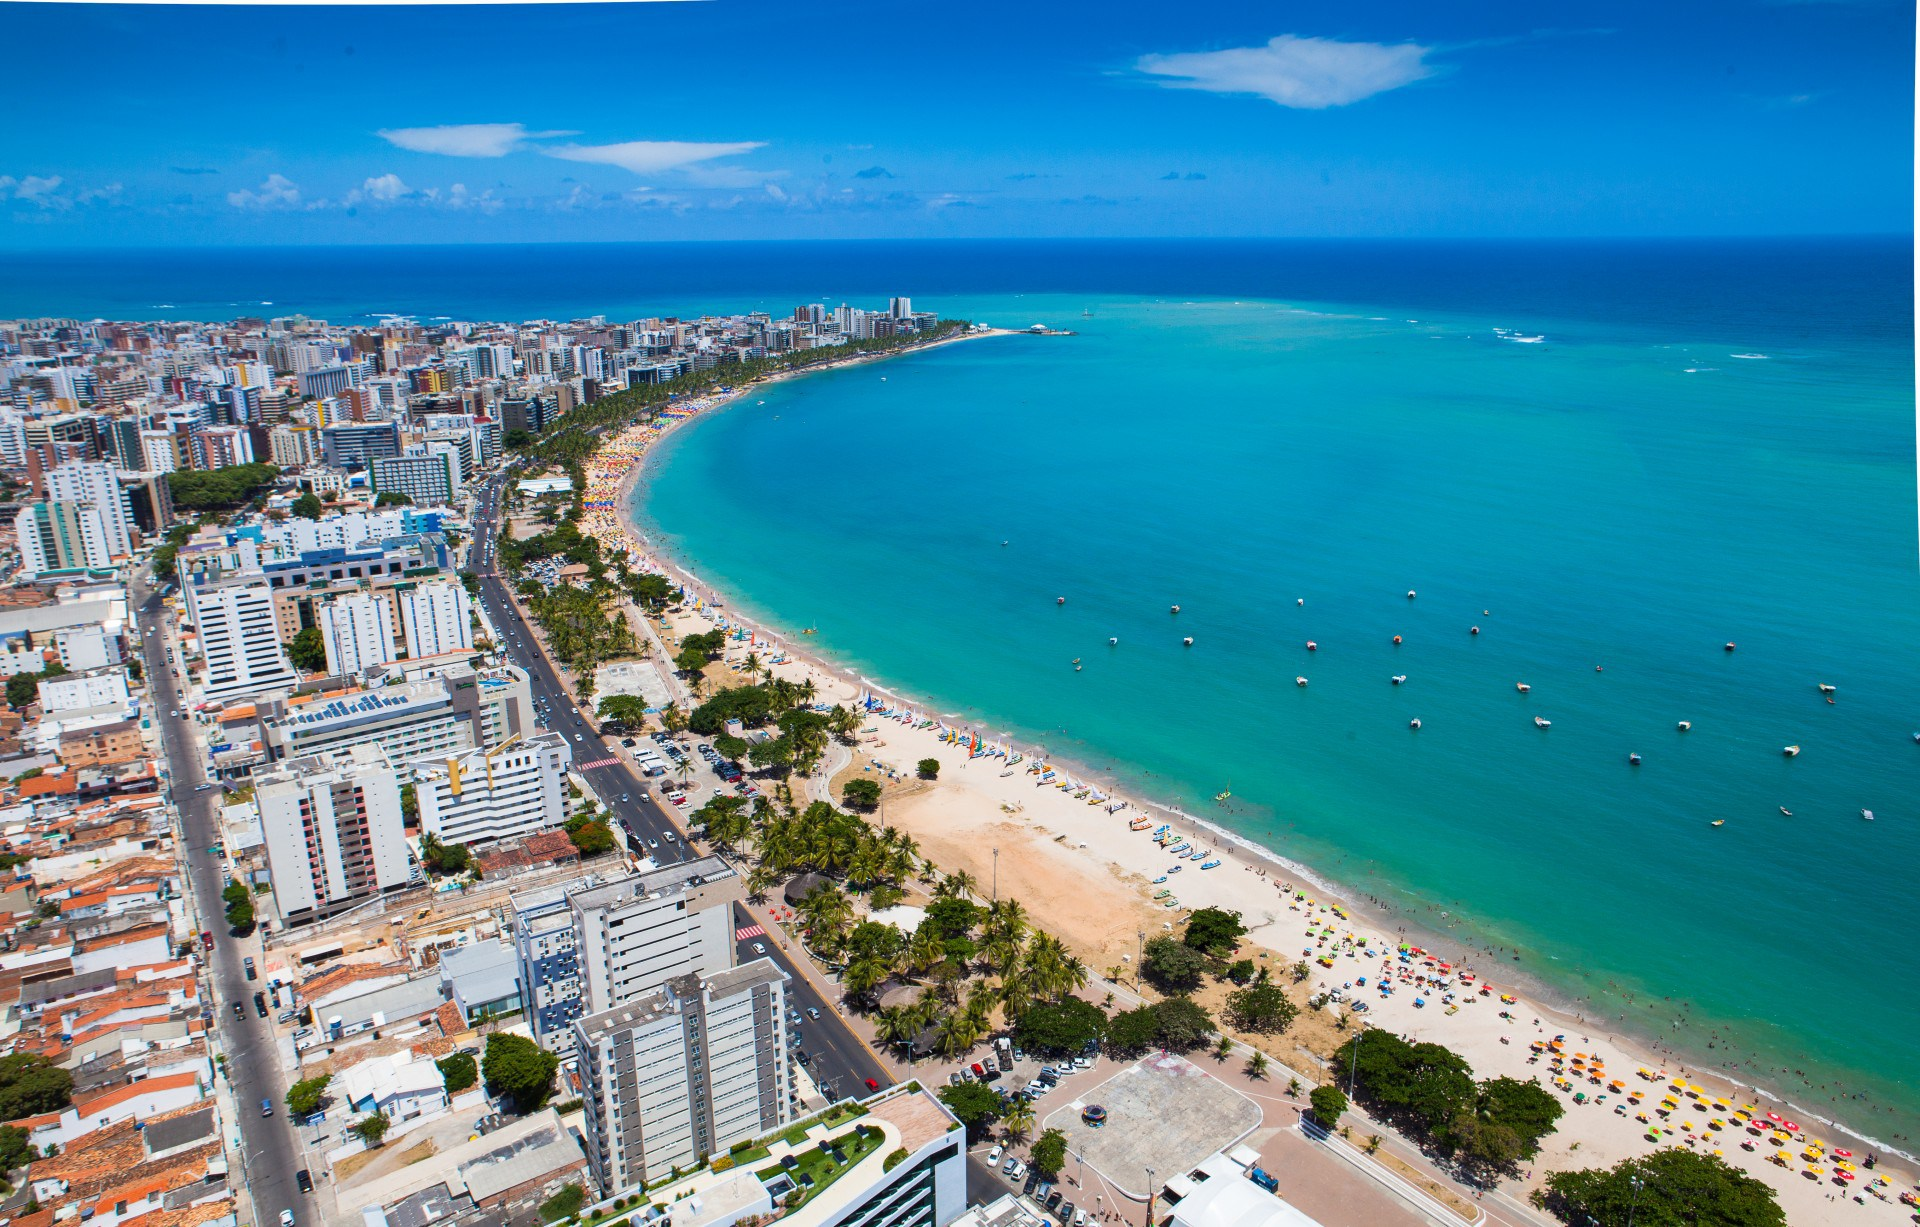
\includegraphics[scale=0.1]{maceio.jpg}
\end{figure}

\section{Tabelas}
\begin{tabular}{|c|c|}
    \hline
    a & b \\
    \hline
    c & d \\
    \hline
\end{tabular}

\section{Sistemas lineares}

\end{document}
